\section{Multivariable analysis}

\subsection{Samples}
Signal samples:
\begin{itemize}
\item mc15\_13TeV.392415.MGPy8EG\_A14N23LO\_C1N2\_Slep\_400\_300\_0p95\_2L5.merge.DAOD\_SUSY2.e4287\_a766\_a810\_r6282\_p2499\_p2500\_pUM999999
\end{itemize}

Background samples:

Charge flip and fake lepton background are data driven. The GRL $data15_13TeV.periodAllYear_DetStatus-v73-pro19-08_DQDefects-00-01-02_PHYS_StandardGRL_All_Good_25ns.xml$ was used. The 3.2fb-1 data used contains the following run numbers:
\begin{itemize}
\item 276262
\item 276329
\item 276336
\item 276416
\item 276511
\item 276689
\item 276778
\item 276790
\item 276952
\item 276954
\item 278880
\item 278912
\item 278968
\item 279169
\item 279259
\item 279279
\item 279284
\item 279345
\item 279515
\item 279598
\item 279685
\item 279764
\item 279813
\item 279867
\item 279928
\item 279932
\item 279984
\item 280231
\item 280319
\item 280368
\item 280423
\item 280464
\item 280500
\item 280520
\item 280614
\item 280673
\item 280753
\item 280853
\item 280862
\item 280950
\item 280977
\item 281070
\item 281074
\item 281075
\item 281317
\item 281385
\item 281411
\item 282625
\item 282631
\item 282712
\item 282784
\item 282992
\item 283074
\item 283155
\item 283270
\item 283429
\item 283608
\item 283780
\item 284006
\item 284154
\item 284213
\item 284285
\item 284420
\item 284427
\item 284484
\end{itemize}
Wgamma, diboson and ttbar background are from following MC samples:\\
\begin{itemize}
\item 410066	MadGraphPythia8EvtGen\_A14NNPDF23LO\_ttW\_Np0
\item 410067	MadGraphPythia8EvtGen\_A14NNPDF23LO\_ttW\_Np1
\item 410068	MadGraphPythia8EvtGen\_A14NNPDF23LO\_ttW\_Np2
\item 410112	MadGraphPythia8EvtGen\_A14NNPDF23LO\_ttee\_Np1
\item 410115	MadGraphPythia8EvtGen\_A14NNPDF23LO\_tttautau\_Np0
\item 410114	MadGraphPythia8EvtGen\_A14NNPDF23LO\_ttmumu\_Np1
\item 410113	MadGraphPythia8EvtGen\_A14NNPDF23LO\_ttmumu\_Np0
\item 410111	MadGraphPythia8EvtGen\_A14NNPDF23LO\_ttee\_Np0
\item 410116	MadGraphPythia8EvtGen\_A14NNPDF23LO\_tttautau\_Np1
\item 361063	Sherpa\_CT10\_llll
\item 361064	Sherpa\_CT10\_lllvSFMinus
\item 361065	Sherpa\_CT10\_lllvOFMinus
\item 361066	Sherpa\_CT10\_lllvSFPlus
\item 361067	Sherpa\_CT10\_lllvOFPlus
\item 361068	Sherpa\_CT10\_llvv
\item 361069	Sherpa\_CT10\_llvvjj\_ss\_EW4
\item 361070	Sherpa\_CT10\_llvvjj\_ss\_EW6
\item 361071	Sherpa\_CT10\_lllvjj\_EW6
\item 361072	Sherpa\_CT10\_lllljj\_EW6
\item 301890	Sherpa\_CT10\_enugammaPt35\_70
\item 301891	Sherpa\_CT10\_enugammaPt70\_140
\item 301892	Sherpa\_CT10\_enugammaPt140
\item 301893	Sherpa\_CT10\_munugammaPt35\_70
\item 301894	Sherpa\_CT10\_munugammaPt70\_140
\item 301895	Sherpa\_CT10\_munugammaPt140
\item 301896	Sherpa\_CT10\_taunugammaPt35\_70
\item 301897	Sherpa\_CT10\_taunugammaPt70\_140
\item 301898	Sherpa\_CT10\_taunugammaPt140
\end{itemize}

Data Selection:\\
The follow filters are applied to the data 
\begin{description}


\item [nPrimaryVertex>0] a Vertex need 2+ tracks with pT 2+GeV to be accepted as a primaryVertex
\item [GRL]
\item [“Standard” object definition] \ \\
Tight e TightLLH, Et<20GeV, eta<2.47 \\
Tight mu Medium, pT<25GeV, eta<2.7 \\
and others\\

\item [Exactly 2 lepton]
\item [triggerCut] \ \\

muonTrig =["HLT\_mu26\_imedium", "HLT\_mu24\_imedium", "HLT\_mu24\_iloose\_L1MU15","HLT\_mu20\_iloose\_L1MU15", "HLT\_mu50", "HLT\_mu60\_0eta105\_msonly"]\\

dimuonTrig = ["HLT\_2mu14","HLT\_2mu10","HLT\_mu24\_mu8noL1","HLT\_mu22\_mu8noL1","HLT\_mu20\_mu8noL1","HLT\_mu18\_mu8noL1"]\\

trimuonTrig = ["HLT\_mu24\_2mu4noL1","HLT\_mu22\_2mu4noL1","HLT\_mu20\_2mu4noL1","HLT\_mu18\_2mu4noL1","HLT\_3mu6","HLT\_3mu6\_msonly"]\\

electronTrigCut = ["HLT\_e26\_tight\_iloose","HLT\_e60\_medium","HLT\_e24\_tight\_iloose","HLT\_e24\_medium\_iloose\_L1EM20VH","HLT\_e24\_medium\_iloose\_L1EM18VH"]\\

electronTrigLH = ["HLT\_e26\_lhtight\_iloose","HLT\_e60\_lhmedium","HLT\_e24\_lhtight\_iloose","HLT\_e24\_lhmedium\_iloose\_L1EM20VH","HLT\_e24\_lhmedium\_iloose\_L1EM18VH"]\\

dielectronTrigCut = ["HLT\_2e17\_loose","HLT\_2e15\_loose\_L12EM13VH","HLT\_2e12\_loose\_L12EM10VH"]\\

dielectronTrigLH = ["HLT\_2e17\_lhloose","HLT\_2e15\_lhloose\_L12EM13VH","HLT\_2e12\_lhloose\_L12EM10VH"]\\

trielectronTrigCut = ["HLT\_e17\_medium\_2e9\_medium"]\\

trielectronTrigLH = ["HLT\_e17\_lhmedium\_2e9\_lhmedium"]\\

elemuonTrigCut = ["HLT\_e17\_loose\_mu14","HLT\_e7\_medium\_mu24","HLT\_e26\_medium\_L1EM22VHI\_mu8noL1","HLT\_e24\_medium\_L1EM20VHI\_mu8noL1"]\\

elemuonTrigLH = ["HLT\_e17\_lhloose\_mu14","HLT\_e7\_lhmedium\_mu24","HLT\_e26\_lhmedium\_L1EM22VHI\_mu8noL1","HLT\_e24\_lhmedium\_L1EM20VHI\_mu8noL1"]\\

trielemuonTrigCut = ["HLT\_e12\_loose\_2mu10","HLT\_2e12\_loose\_mu10"]\\

trielemuonTrigLH = ["HLT\_e12\_lhloose\_2mu10","HLT\_2e12\_lhloose\_mu10"]\\

\item [0 Bjet]\ \\
\item [0 cosmic mu]\ \\
\end{description}


\subsection{Variables}
BDT Training:\\
We separate out two event types, the ISR region is defined as events having >=1 jets, and the nonISR region which are events eith no jets.

In both region we train a Boosted Decision Tree to classifying out signal event from background. The BDTD algo in ROOT's TMVA package was used for the job, where BDTD stands for Boosted Decision Tree with decorrelated variables. 

In the nonISR region the following variables are used as input:
\begin{itemize}
\item mT2
\item $pT_{dilepton}$
\item $E_{T}^{Miss,rel}$
\item $H_T$ (scalar sum for 2l+jets pT)
\item $m_{T,l1}$ (transvers mass with leading lepton)
\item $m_{T,l2}$ (transvers mass with 2nd leading lepton)
\item $dPhi_{(l1,l2)}$
\item l12m(dilepton mass)

\end{itemize}

In the ISR region the following extra variables are also used:
\begin{itemize}
\item $dPhi_{(Etmissrel,leading jet)}$
\item $E_T^{miss,rel}/p_{T,leading jet}$
\item $p_{T,l1}/p_{T,leading jet}$
\end{itemize}

The correlation of the BDT input variables for signal and background samples are show in fig\ref{fig:BDT_input_corr}

\begin{figure}
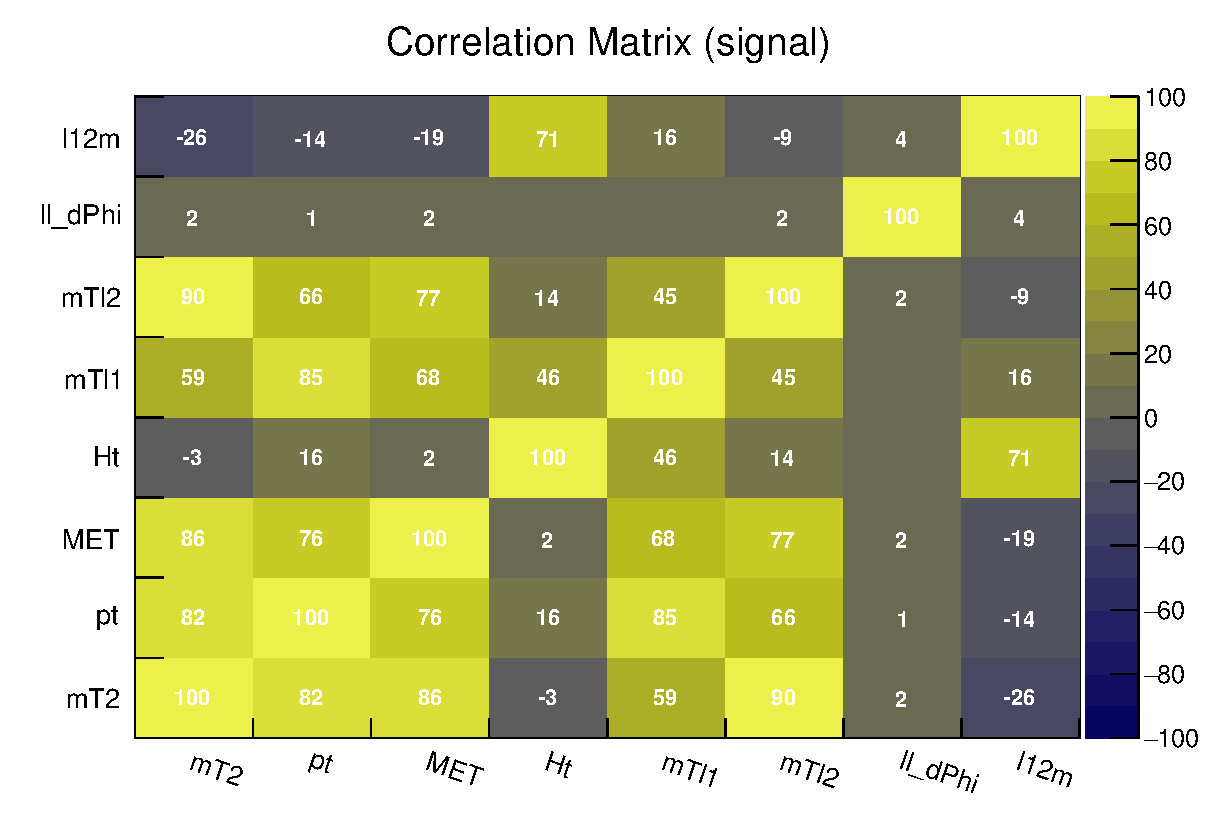
\includegraphics[width=0.5\textwidth]{cutOpt/corrMatS.eps}
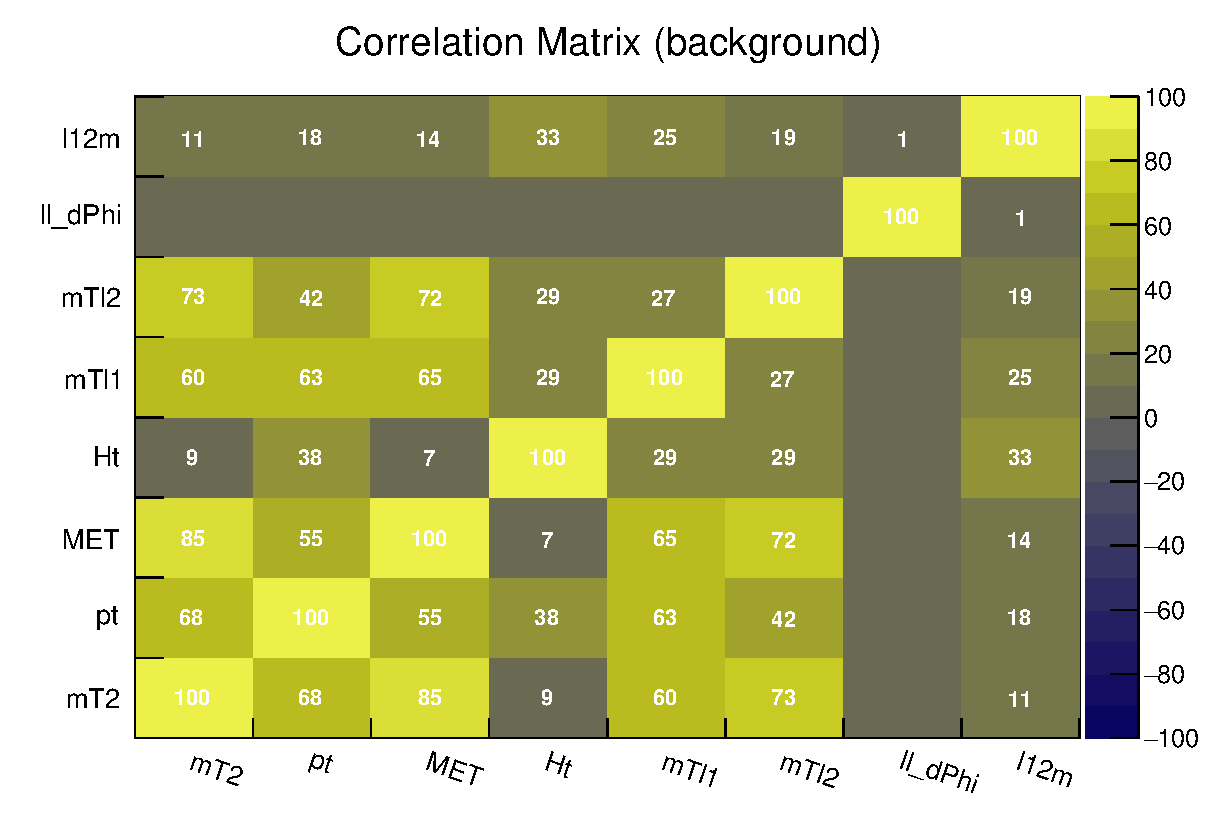
\includegraphics[width=0.5\textwidth]{cutOpt/corrMatB.eps}
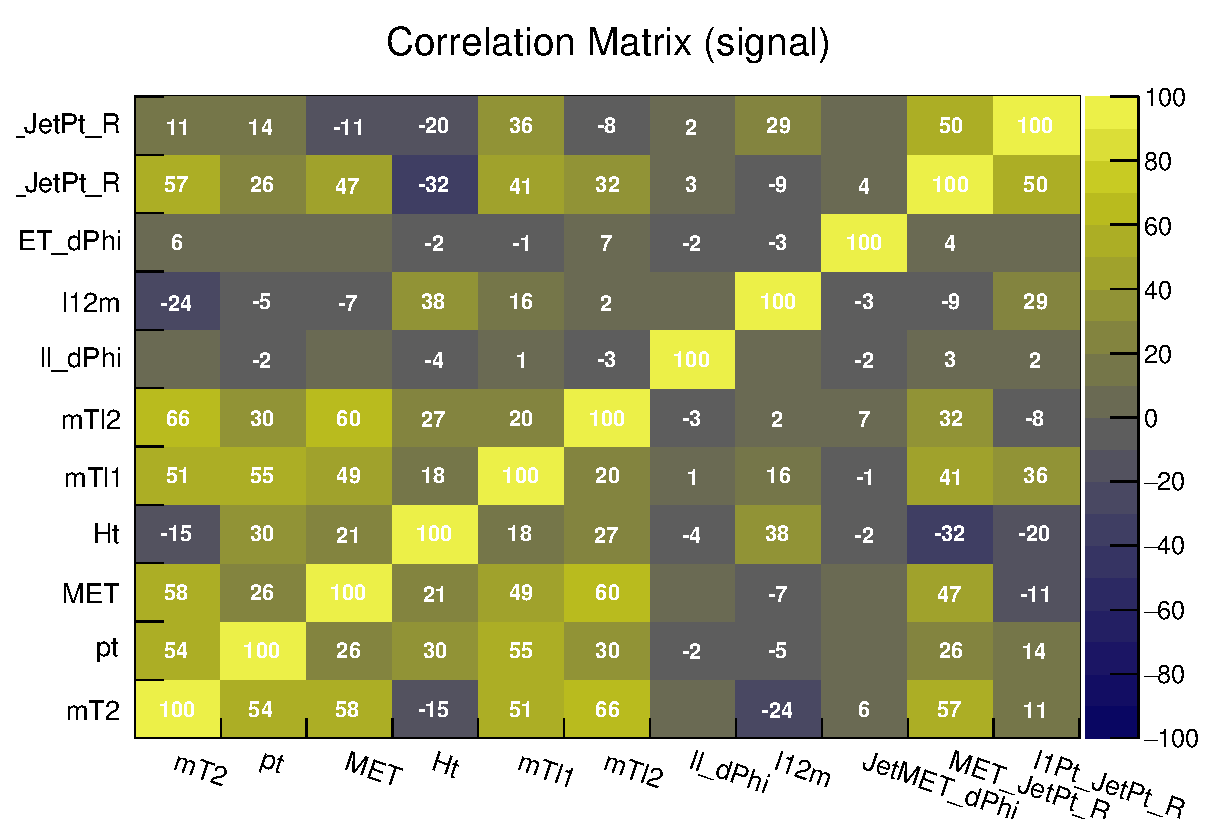
\includegraphics[width=0.5\textwidth]{cutOpt/corrMatS_ISR.eps}
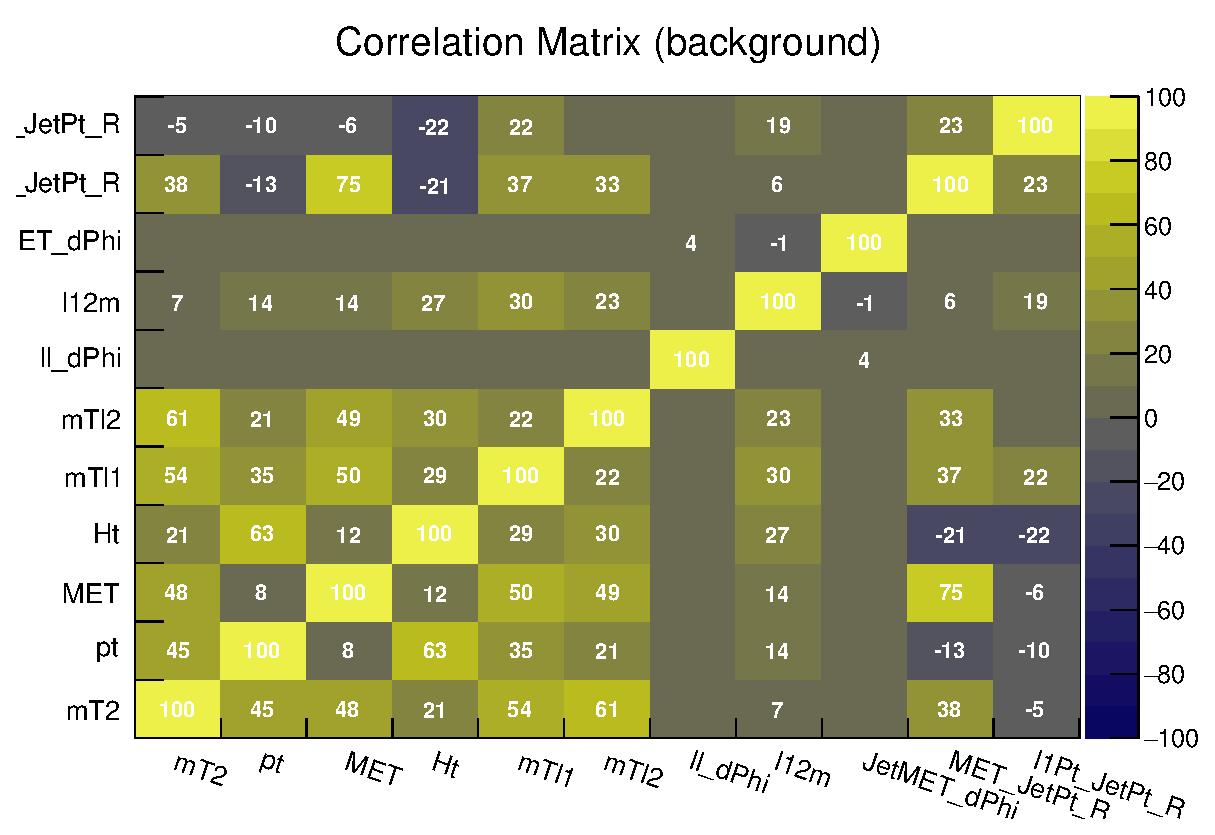
\includegraphics[width=0.5\textwidth]{cutOpt/corrMatB_ISR.eps}
\caption{BDT input variables correlations}
\label{fig:BDT_input_corr}
\end{figure}


The distribution of the BDT input for signal and background samples are show in fig\ref{fig:BDT_nonISR_input}, \ref{fig:BDT_ISR_input}

\begin{figure}
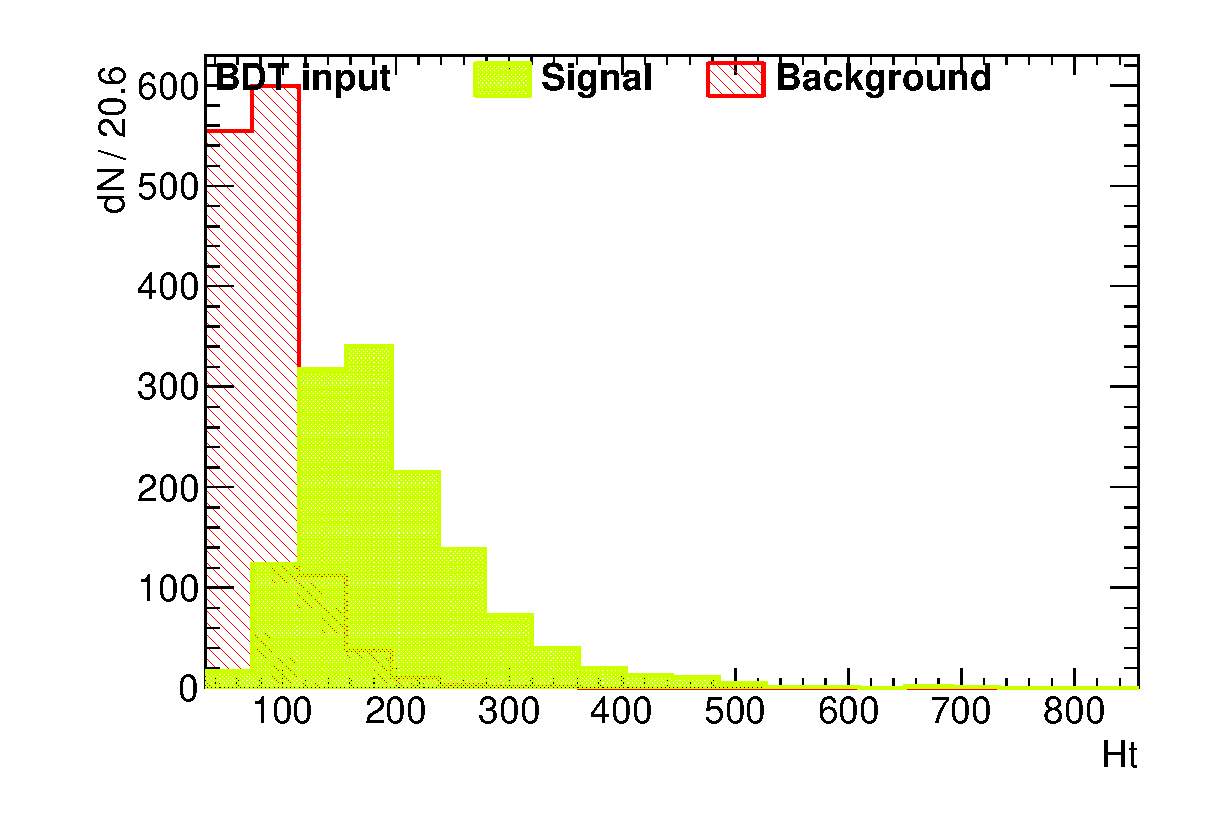
\includegraphics[width=0.5\textwidth]{cutOpt/nonISR_Ht__Signal_Id.eps}
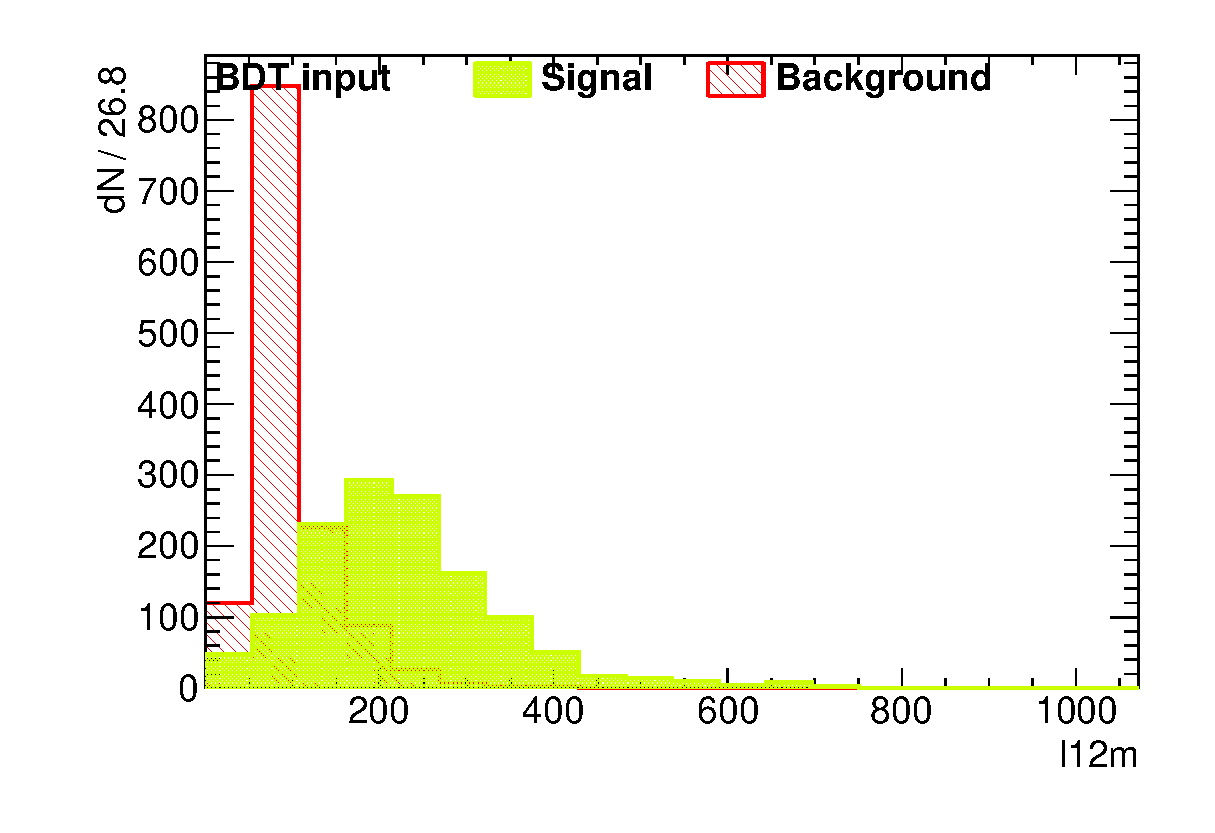
\includegraphics[width=0.5\textwidth]{cutOpt/nonISR_l12m__Signal_Id.eps}
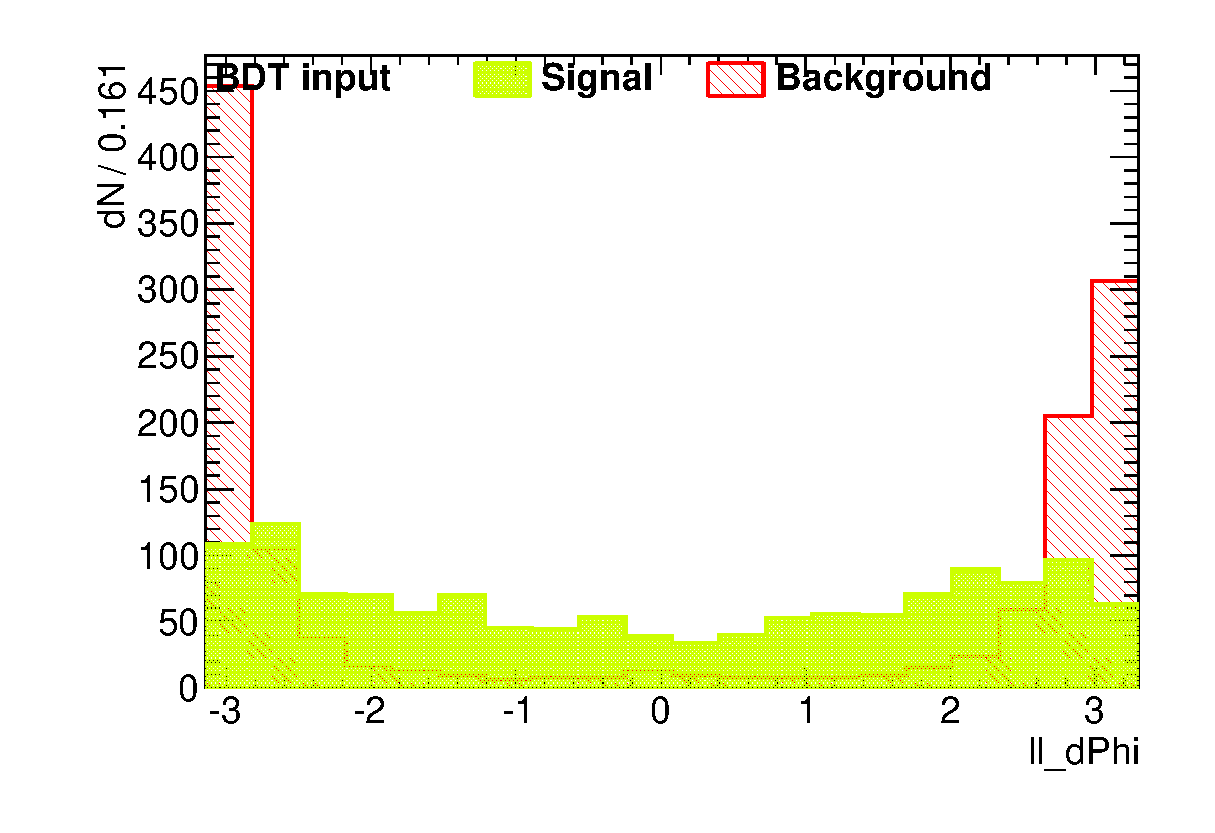
\includegraphics[width=0.5\textwidth]{cutOpt/nonISR_ll_dPhi__Signal_Id.eps}
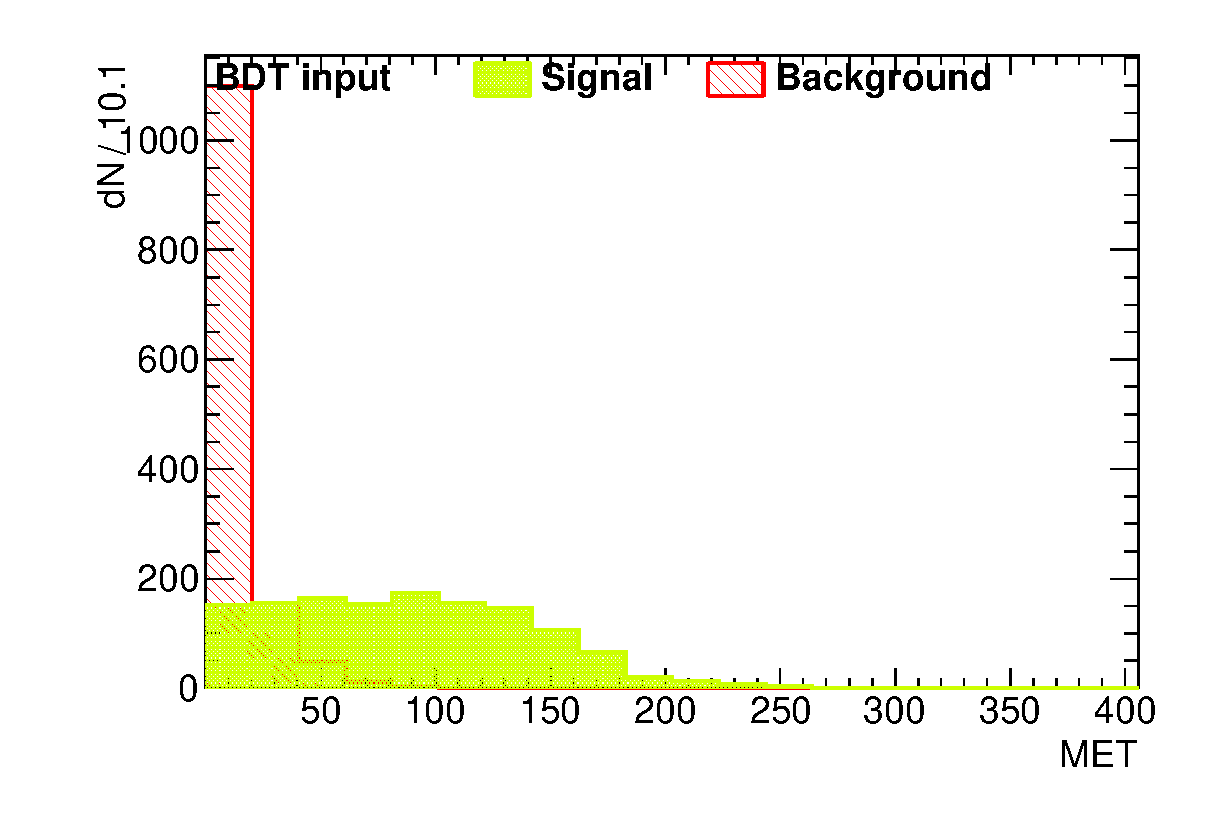
\includegraphics[width=0.5\textwidth]{cutOpt/nonISR_MET__Signal_Id.eps}
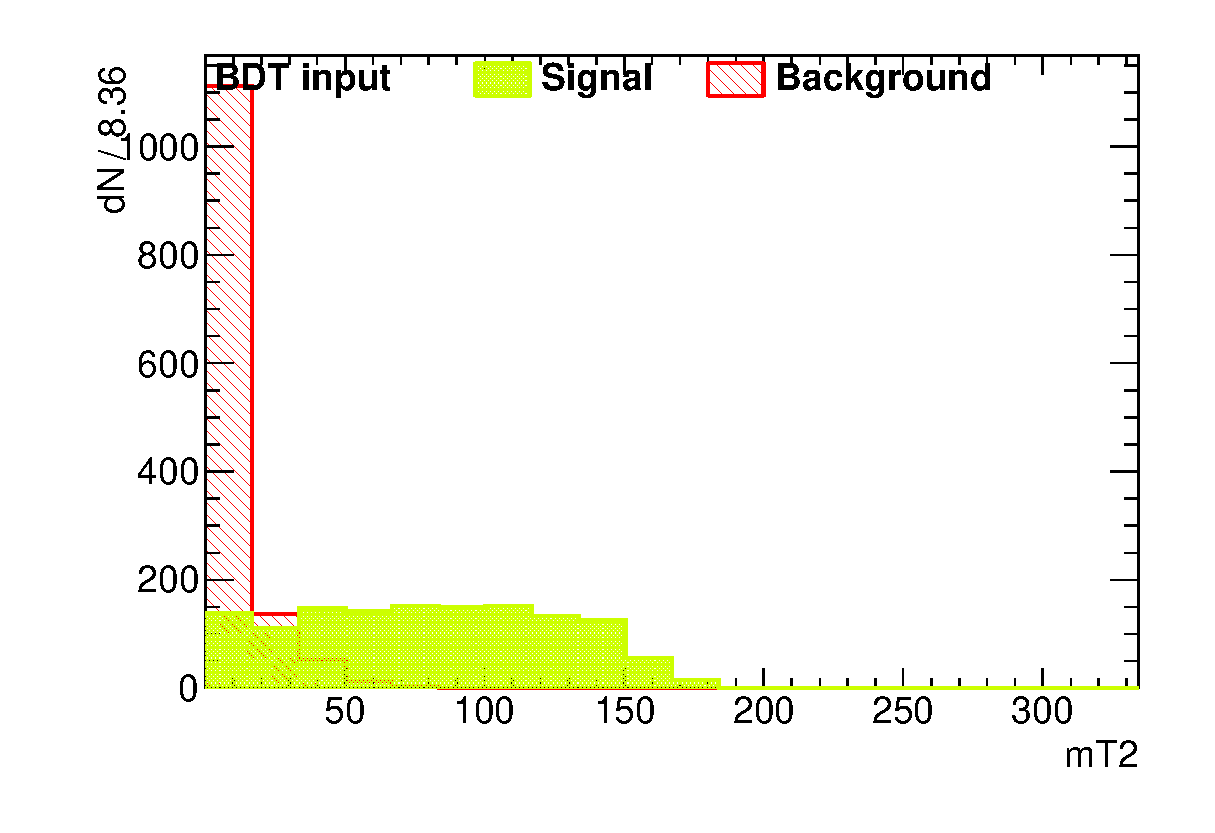
\includegraphics[width=0.5\textwidth]{cutOpt/nonISR_mT2__Signal_Id.eps}
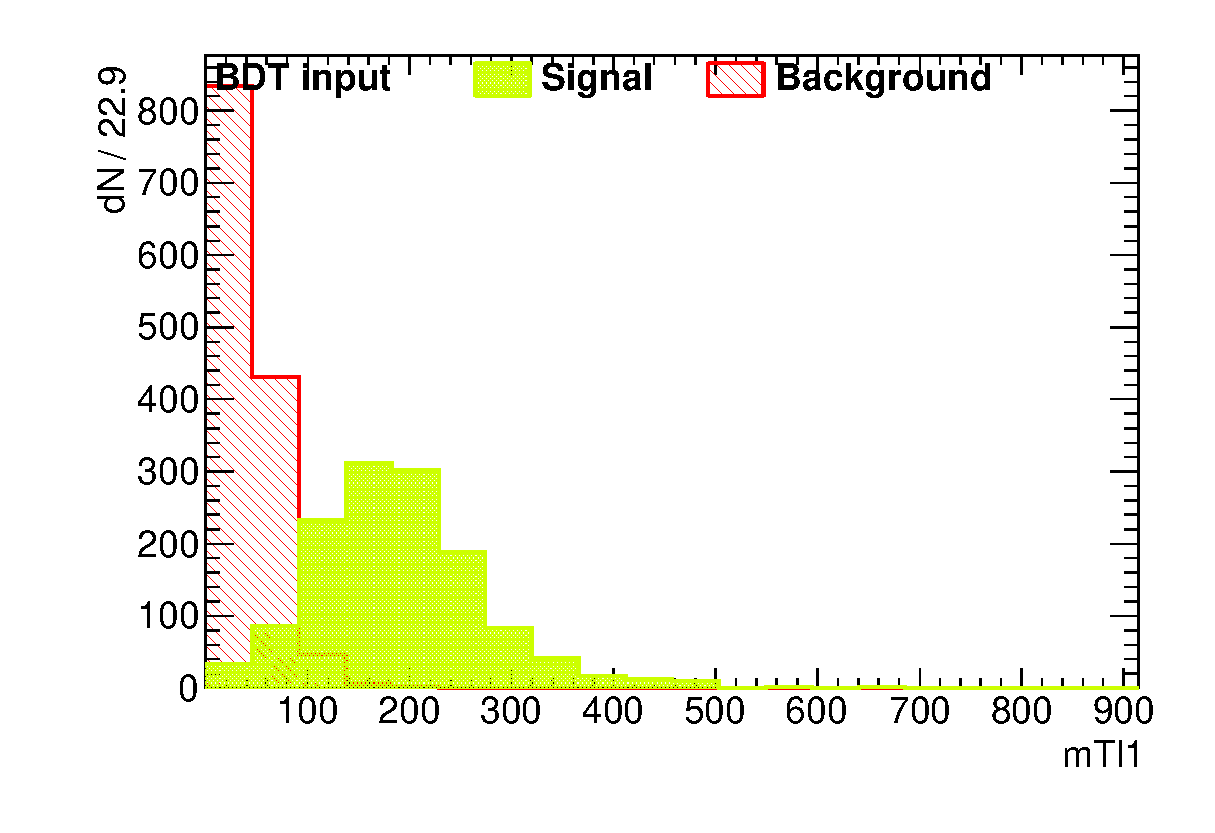
\includegraphics[width=0.5\textwidth]{cutOpt/nonISR_mTl1__Signal_Id.eps}
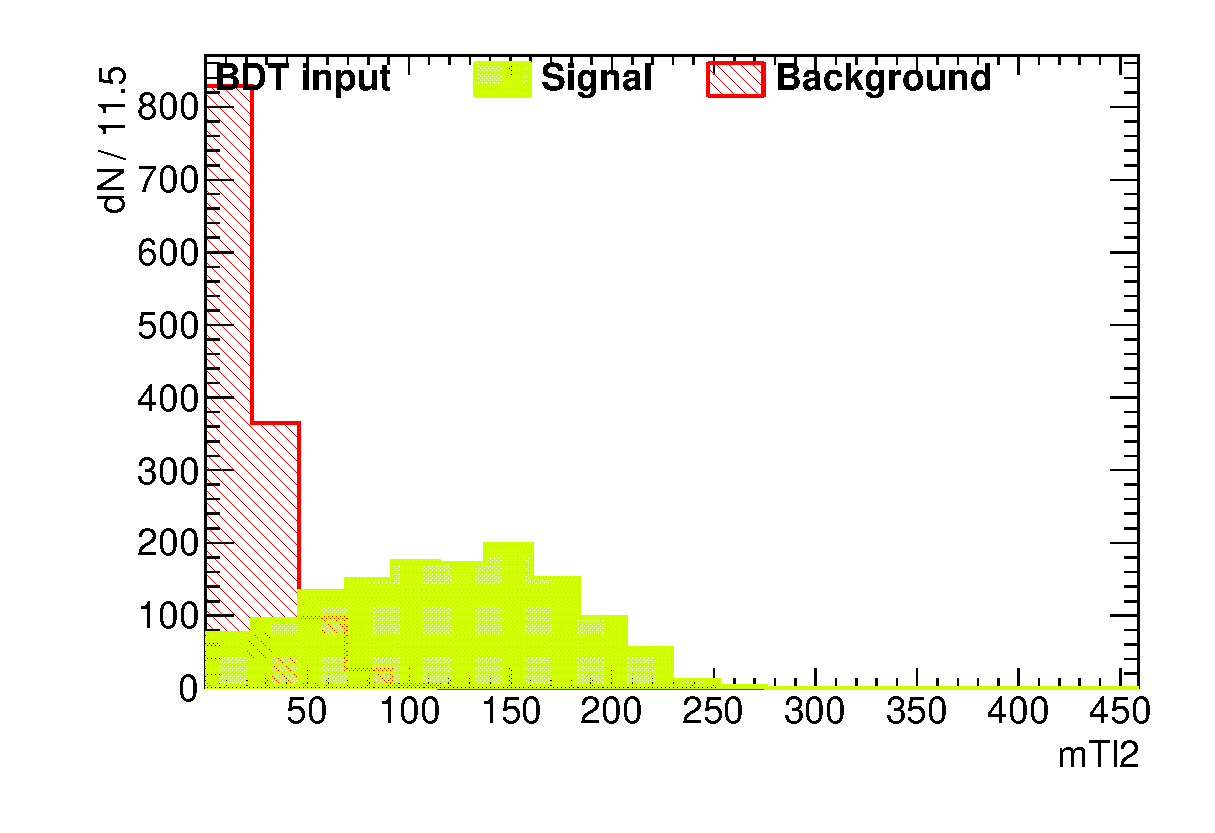
\includegraphics[width=0.5\textwidth]{cutOpt/nonISR_mTl2__Signal_Id.eps}
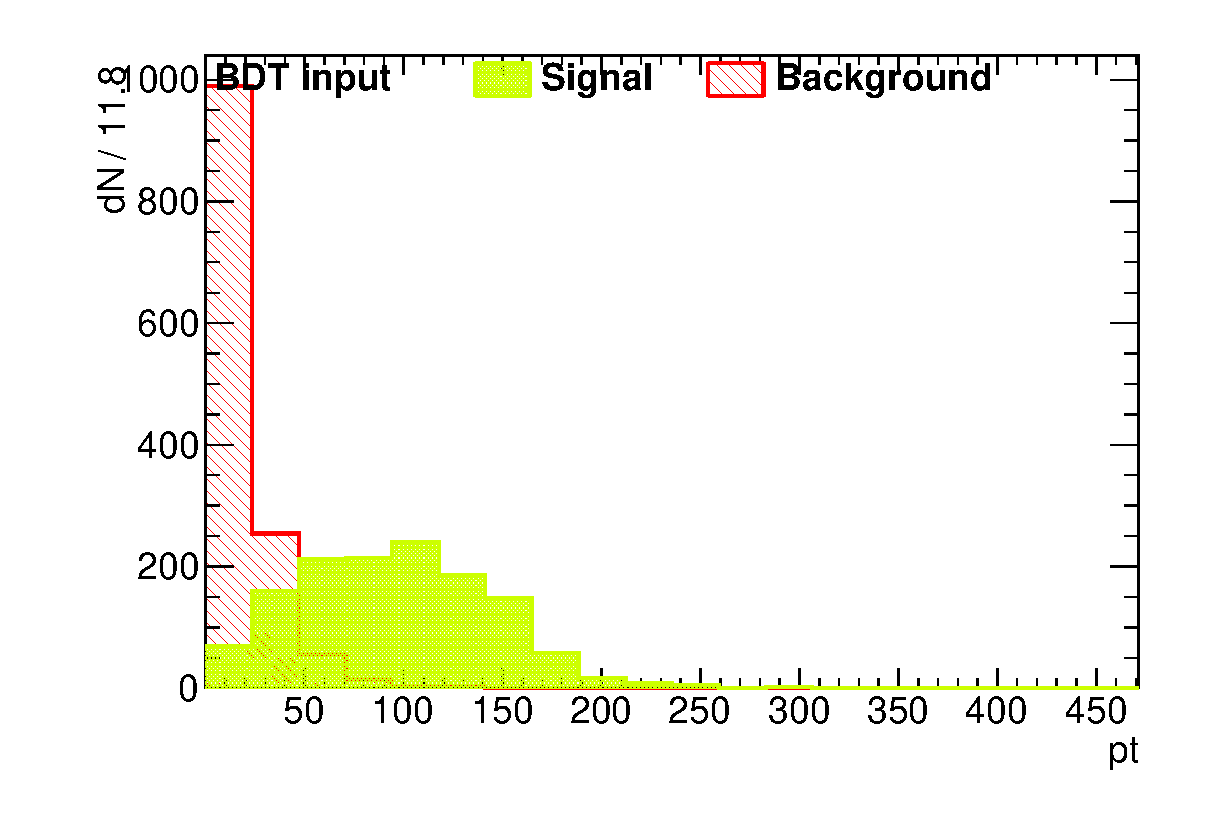
\includegraphics[width=0.5\textwidth]{cutOpt/nonISR_pt__Signal_Id.eps}
\caption{BDT input variables distribution for nonISR region}
\label{fig:BDT_nonISR_input}
\end{figure}

\begin{figure}
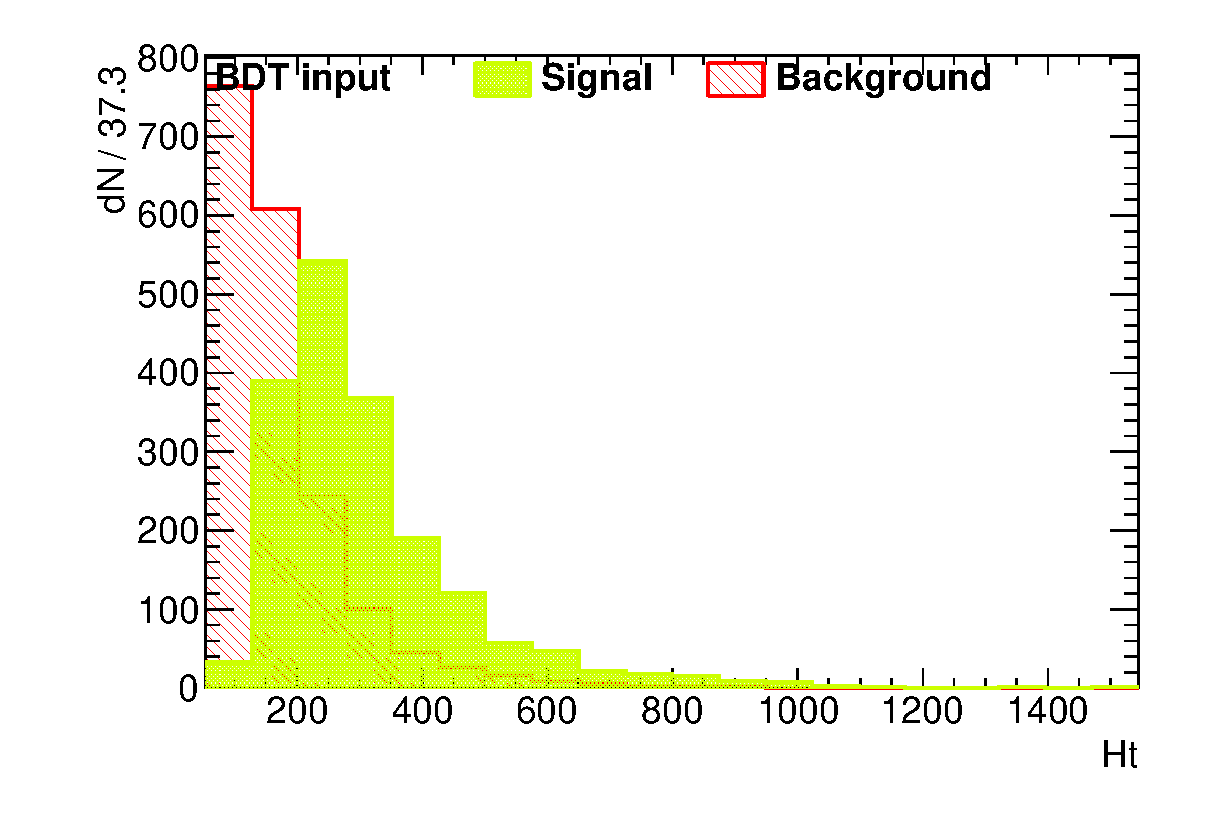
\includegraphics[width=0.5\textwidth]{cutOpt/ISR_Ht__Signal_Id.eps}
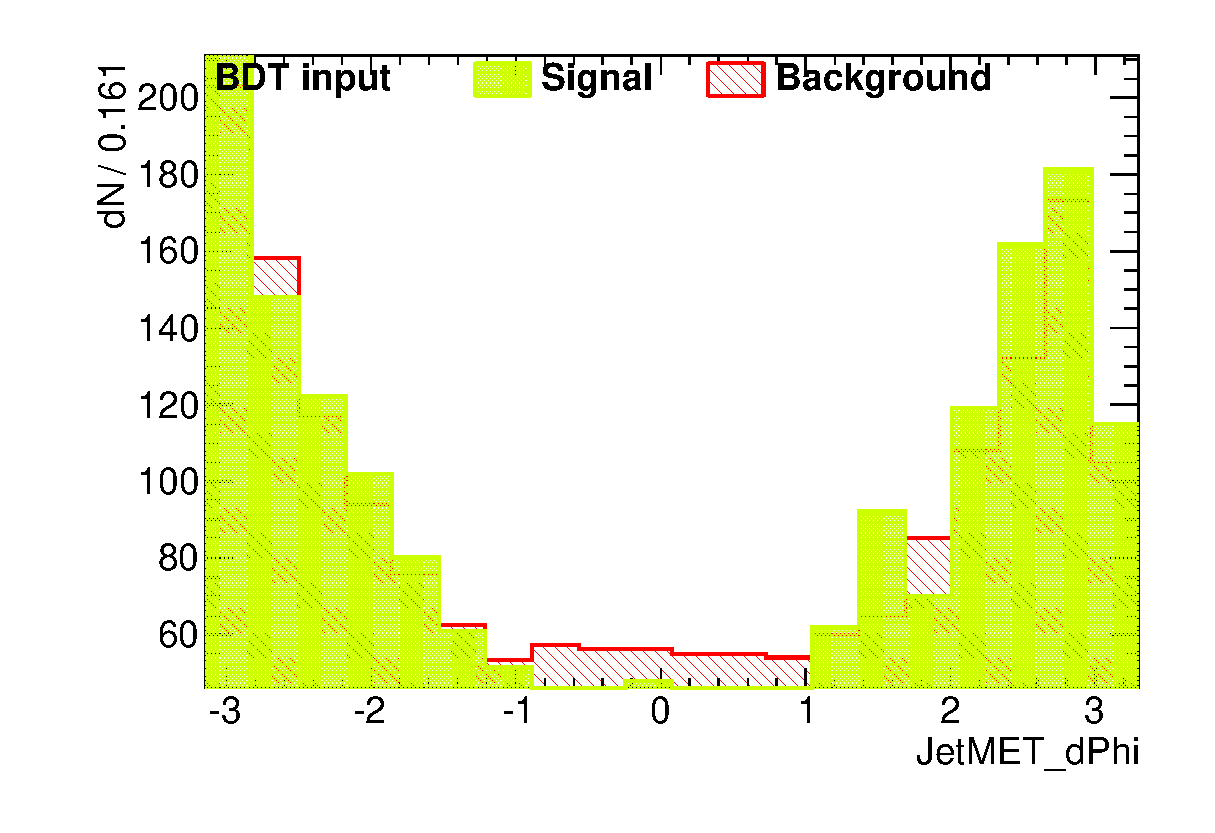
\includegraphics[width=0.5\textwidth]{cutOpt/ISR_JetMET_dPhi__Signal_Id.eps}
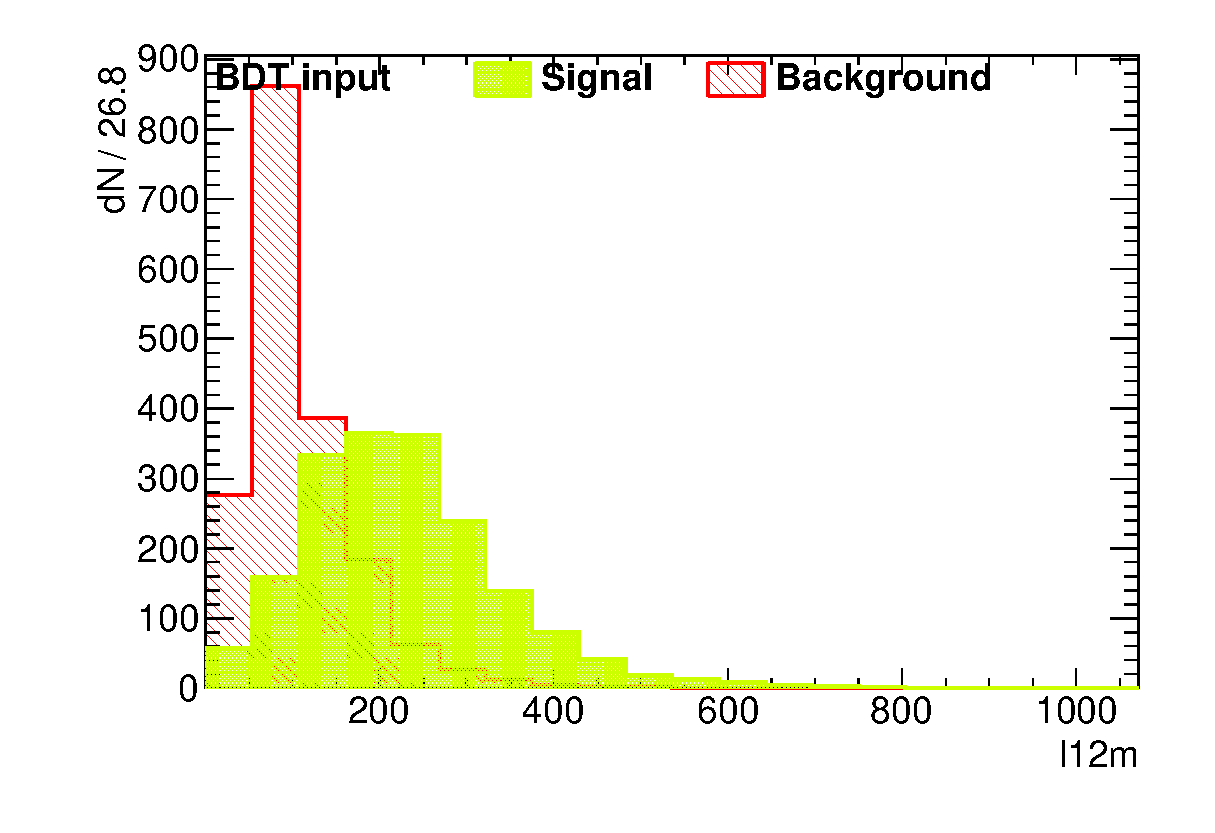
\includegraphics[width=0.5\textwidth]{cutOpt/ISR_l12m__Signal_Id.eps}
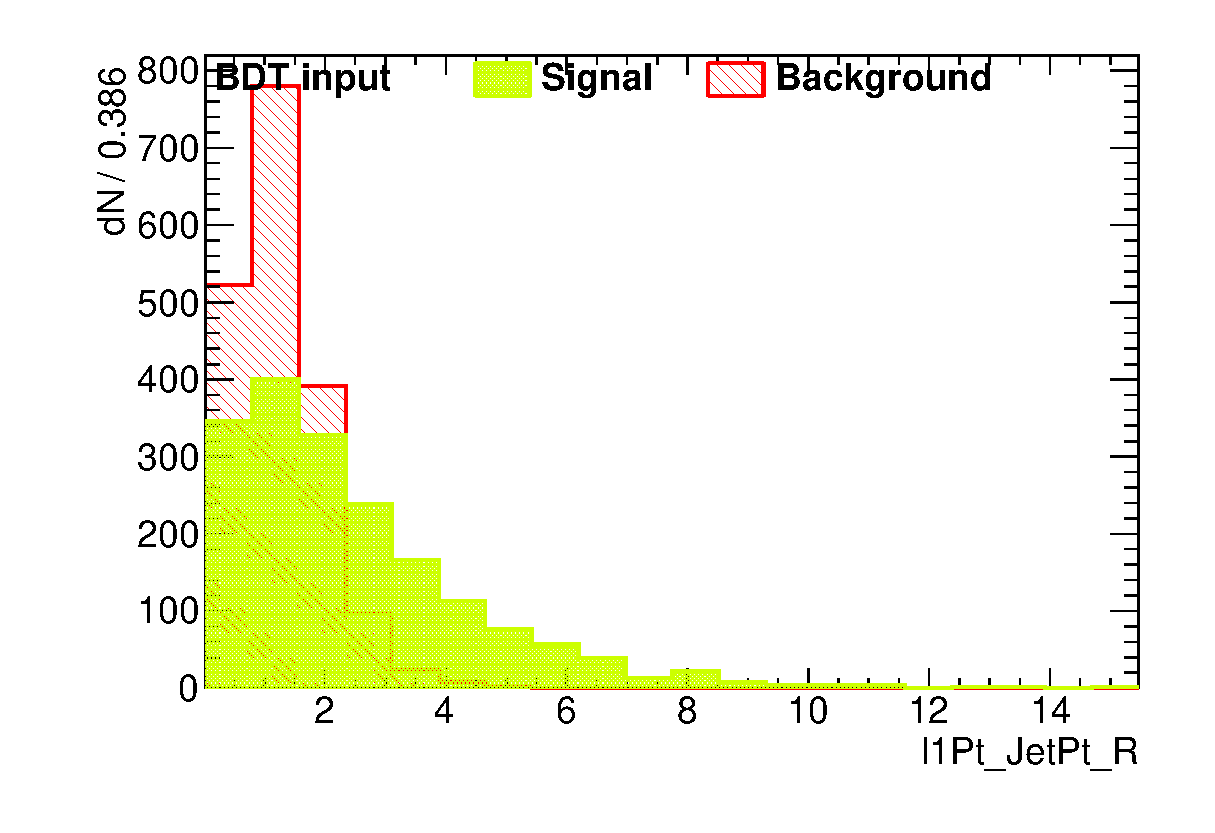
\includegraphics[width=0.5\textwidth]{cutOpt/ISR_l1Pt_JetPt_R__Signal_Id.eps}
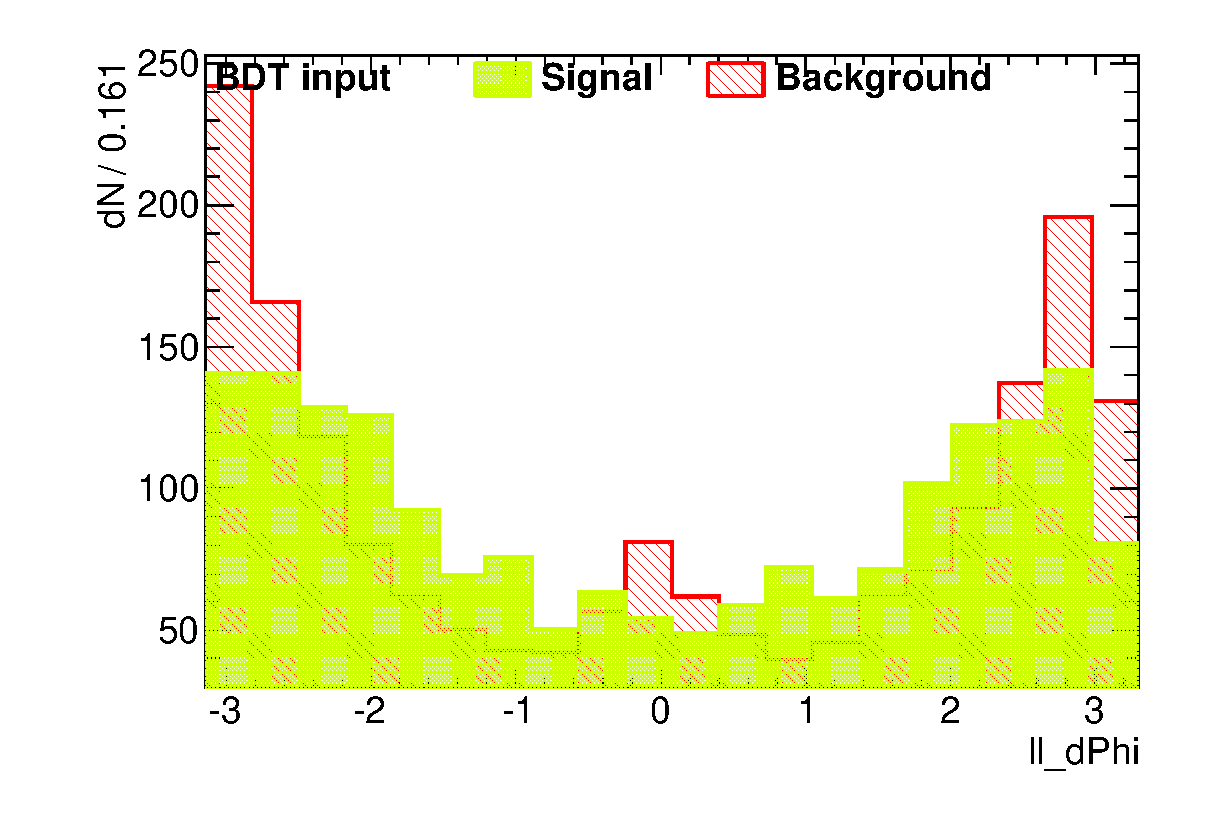
\includegraphics[width=0.5\textwidth]{cutOpt/ISR_ll_dPhi__Signal_Id.eps}
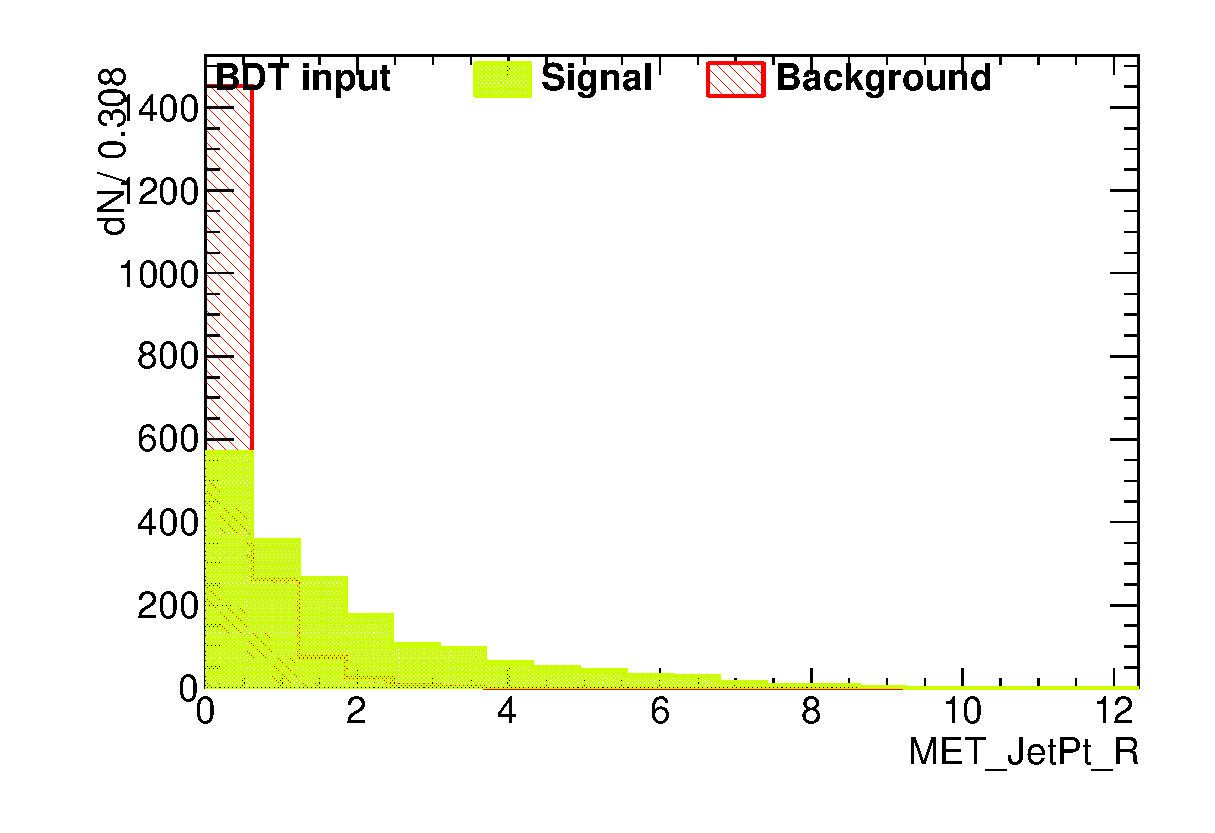
\includegraphics[width=0.5\textwidth]{cutOpt/ISR_MET_JetPt_R__Signal_Id.eps}
\caption{BDT input variables distribution for ISR region}
\label{fig:BDT_ISR_input}
\end{figure}

\begin{figure}
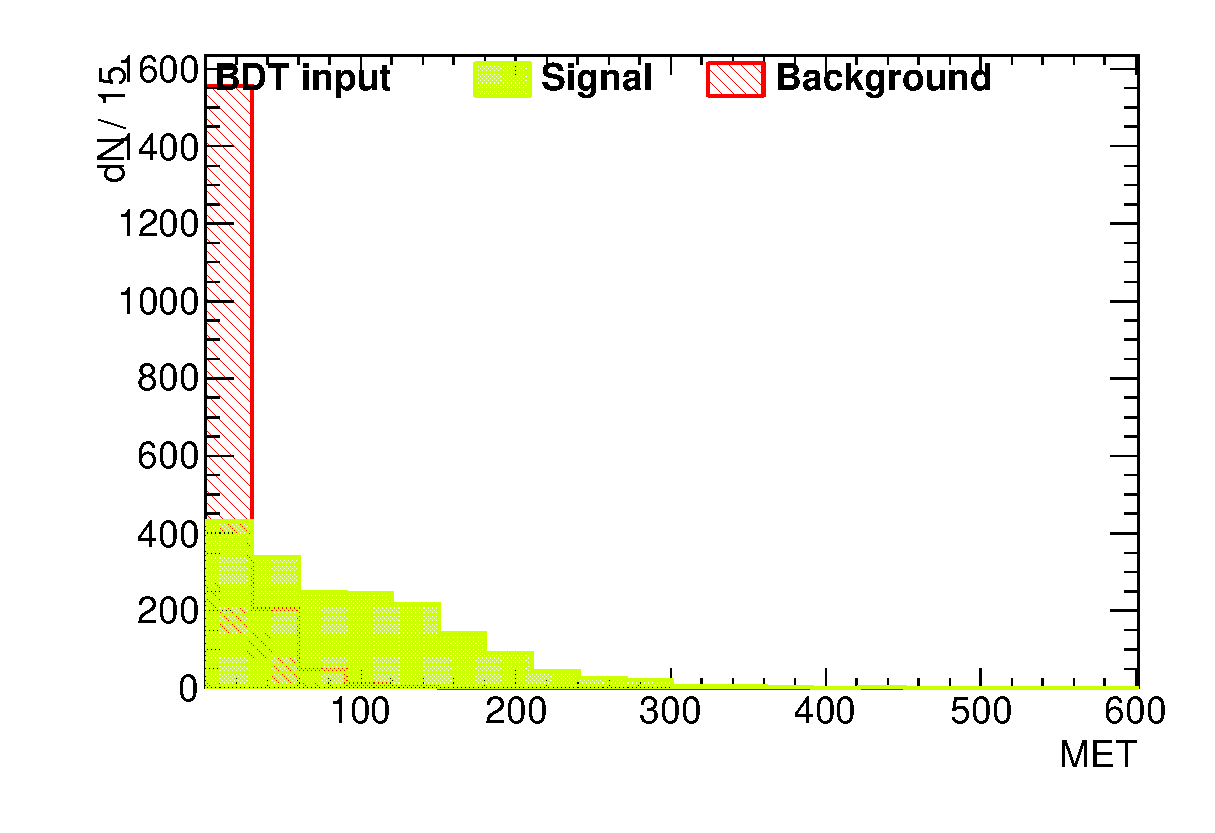
\includegraphics[width=0.5\textwidth]{cutOpt/ISR_MET__Signal_Id.eps}
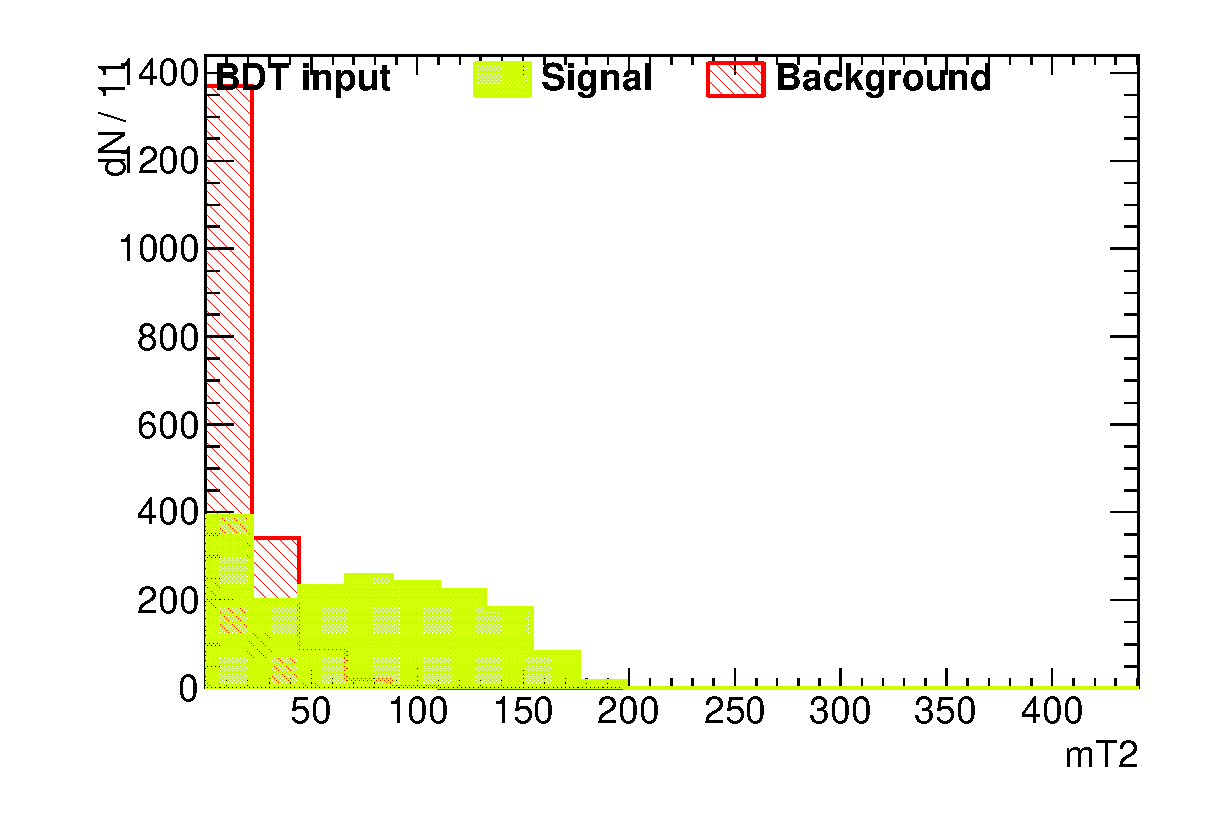
\includegraphics[width=0.5\textwidth]{cutOpt/ISR_mT2__Signal_Id.eps}
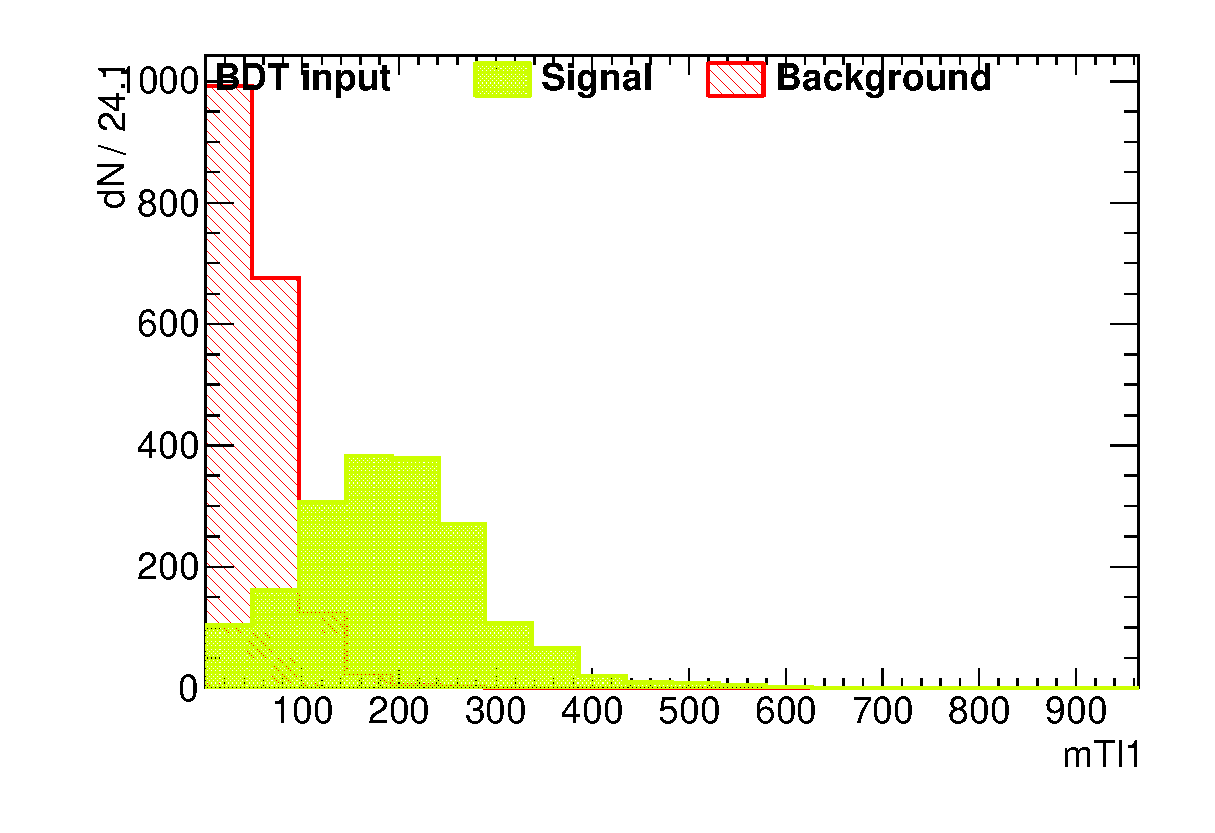
\includegraphics[width=0.5\textwidth]{cutOpt/ISR_mTl1__Signal_Id.eps}
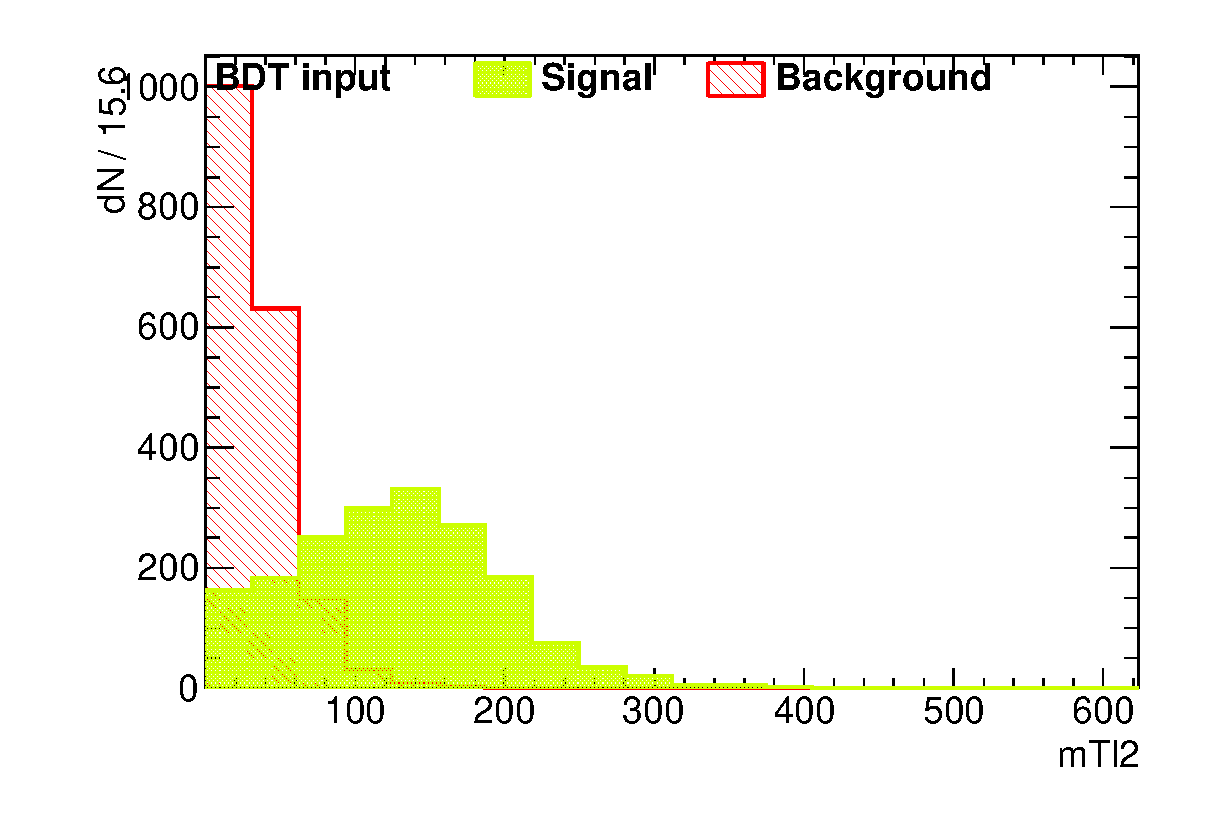
\includegraphics[width=0.5\textwidth]{cutOpt/ISR_mTl2__Signal_Id.eps}
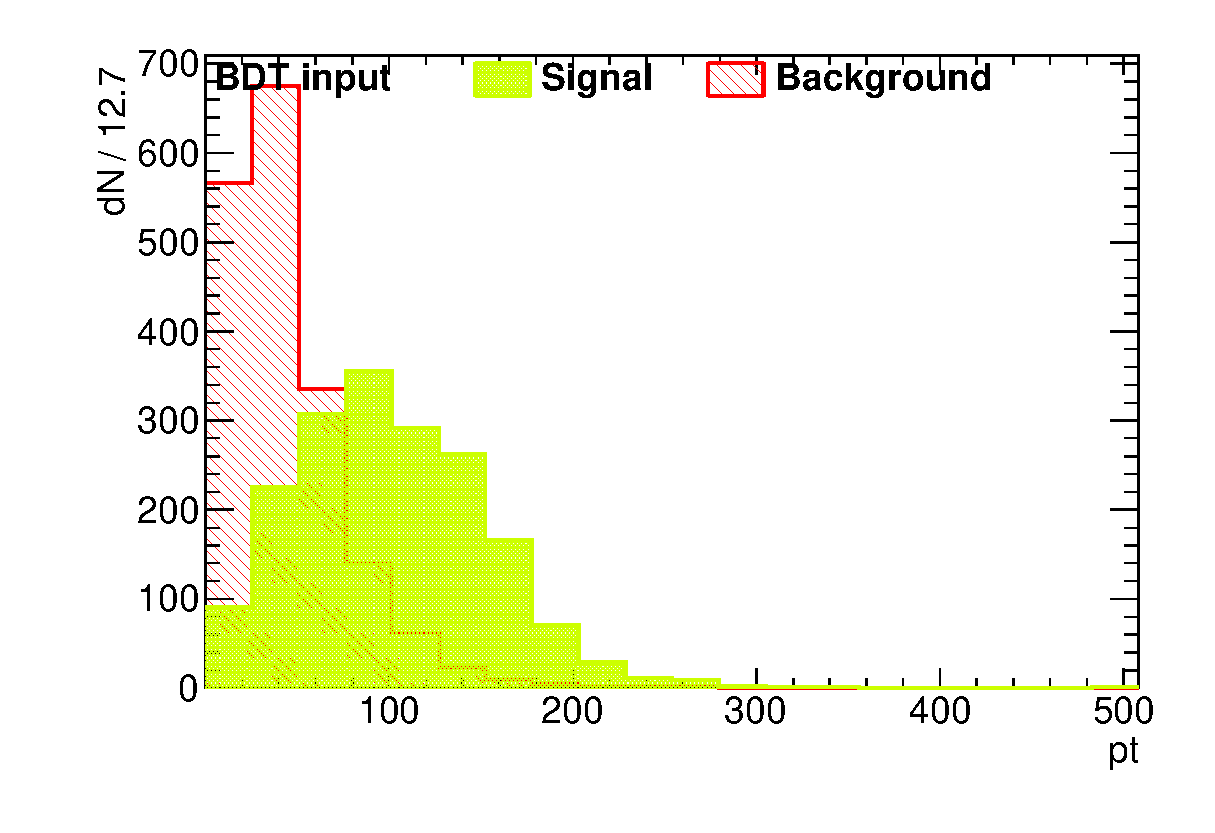
\includegraphics[width=0.5\textwidth]{cutOpt/ISR_pt__Signal_Id.eps}
\caption{BDT input variables distribution for ISR region}
\label{fig:BDT_ISR_input2}
\end{figure}

\subsection{Trainning}
Configuration\\
We have chosen the following setting for the BDTD algo:
\begin{itemize}
\item NTrees=400
\item MinNodeSize=5%
\item MaxDepth=2
\item BoostType=AdaBoost
\item SeparationType=GiniIndex
\item nCuts=20
\item VarTransform=Decorrelate
\end{itemize}
Trainning results:\\
The distribution of the BDT output for signal and background samples are show in fig\ref{fig:BDT_output}

\begin{figure}
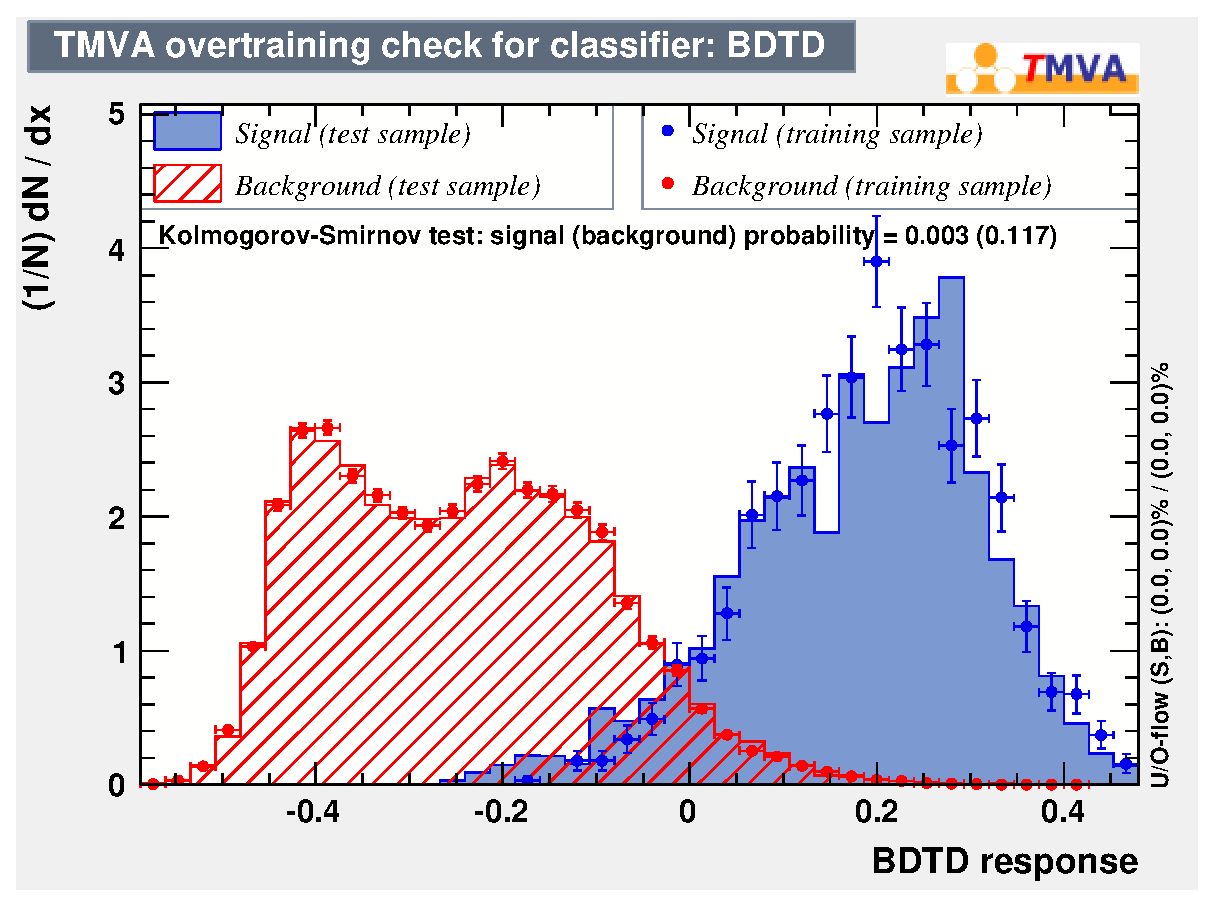
\includegraphics[width=0.5\textwidth]{cutOpt/nonISR_newSample_BDT_dist.eps}
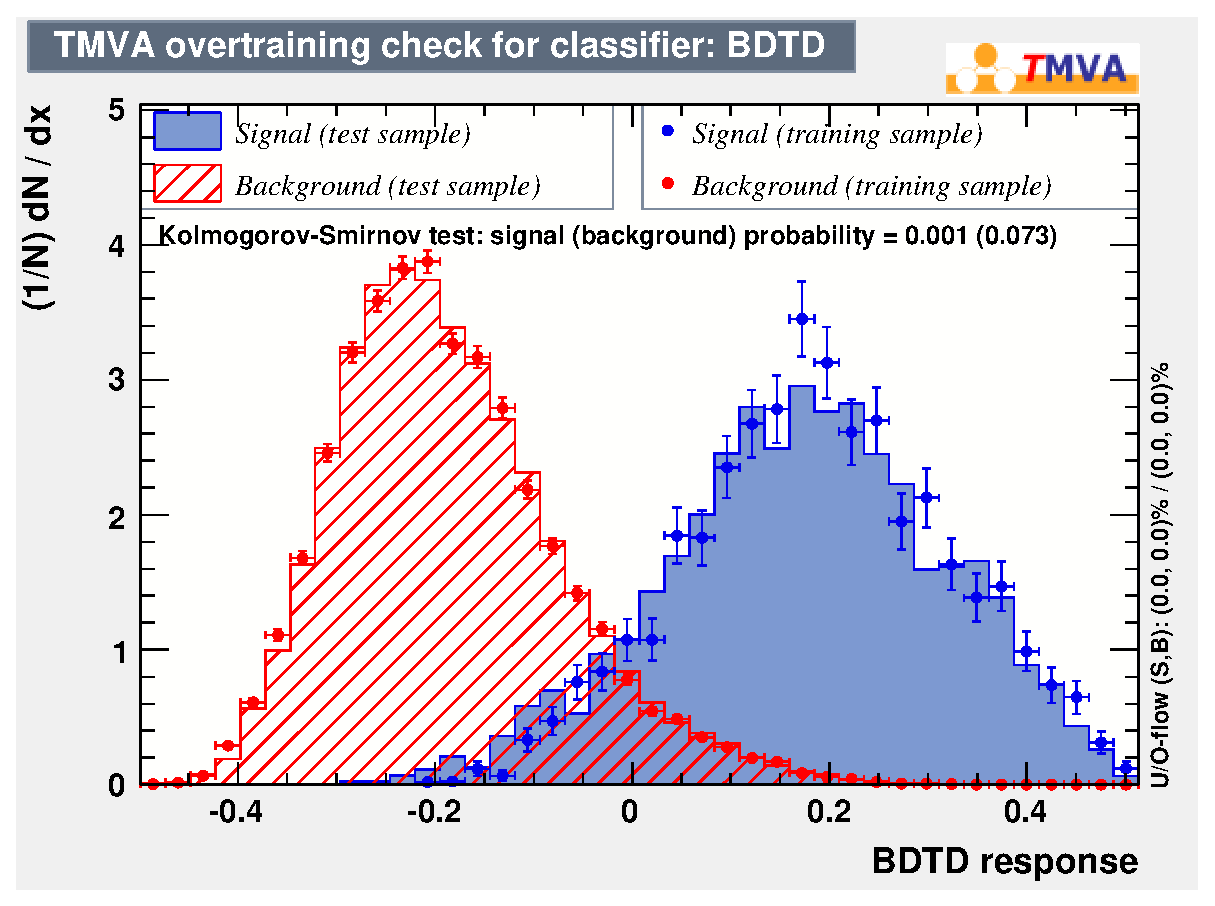
\includegraphics[width=0.5\textwidth]{cutOpt/ISR_newSample_BDT_dist.eps}
\caption{BDT output for nonISR(left) and ISR region(right)}
\label{fig:BDT_output}
\end{figure}

\subsection{Cut optimization}
A cut on BDT output was apllied to define the signal region. Various cut values were tried to find the optimal point. Optimal was defined as having the smallest CLs. To obtain the CLs HistFitter was used. The event counts were projected to 10fb-1 and the expected CLs at that luminosity was calculated. Both the signal region and the control region was blinded during the calculation.

The result shows that the best cut is at 0.25 for nonISR and 0.3 for ISR region.

\begin{table}
\begin{center}
\begin{tabular}{|c|c|c|c|c|c|}
\hline 
BDTcut	&0.2	&0.25	&0.3	&0.35	&0.4 \\
\hline 
CLs	&0.075918	&0.036563	&0.026185	&0.086068	&0.289886\\
CLb	&0.500004	&0.499982	&0.499977	&0.500076	&0.501916\\
CLs+b	&0.037959	&0.018281	&0.013092	&0.043041	&0.145498\\
\hline 
\end{tabular} 
\caption{CLs at various BDT cut for ISR region}
\end{center}
\end{table}

\begin{table}
\begin{center}
\begin{tabular}{|c|c|c|c|}
\hline 
BDTcut	&0.2	&0.25	&0.3\\
\hline 
CLs	&0.128897	&0.103104&	0.215374\\
CLb&	0.500049	&0.499999&	0.500589\\
CLs+b	&0.064455&	0.051552&	0.107814\\
\hline 
\end{tabular} 
\caption{CLs at various BDT cut for nonISR region}
\end{center}
\end{table}
\subsection{Results}
When both regions are combined, a CLs of 0.0034 was obtained.

\begin{table}
\begin{center}
\setlength{\tabcolsep}{0.0pc}
{\small
%%
\begin{tabular*}{\textwidth}{@{\extracolsep{\fill}}lrr}
\noalign{\smallskip}\hline\noalign{\smallskip}
{\bf table.results.yields channel}           & SRISR            & SRnonISR              \\[-0.05cm]
\noalign{\smallskip}\hline\noalign{\smallskip}
%%
Observed events          & $1$              & $7$                    \\
\noalign{\smallskip}\hline\noalign{\smallskip}
%%
Fitted bkg events         & $1.56_{-1.56}^{+1.96}$          & $7.20 \pm 2.57$              \\
\noalign{\smallskip}\hline\noalign{\smallskip}
%%
        Fitted BDT\_MGPy8EG\_A14N23LO\_C1N2\_Slep\_400\_300\_Data\_ events         & $0.05_{-0.05}^{+1.99}$          & $0.06_{-0.06}^{+2.51
}$              \\
%%
        Fitted BDT\_CFlip\_ events         & $0.18 \pm 0.03$          & $0.56 \pm 0.08$              \\
%%
        Fitted BDT\_fakeLep\_ events         & $0.00 \pm 0.00$          & $0.00 \pm 0.00$              \\
%%
        Fitted BDT\_diboson\_Data\_ events         & $1.19 \pm 0.25$          & $3.64 \pm 0.62$              \\
%%
        Fitted BDT\_wgamma\_Data events         & $0.12_{-0.12}^{+0.19}$          & $0.95 \pm 0.25$              \\
%%
        Fitted BDT\_ttbar\_Data\_ events         & $0.03 \pm 0.01$          & $0.01 \pm 0.00$              \\
%%
 \noalign{\smallskip}\hline\noalign{\smallskip}
%%
MC exp. SM events              & $6.93$          & $13.99$              \\
\noalign{\smallskip}\hline\noalign{\smallskip}
%%
        MC exp. BDT\_MGPy8EG\_A14N23LO\_C1N2\_Slep\_400\_300\_Data\_ events         & $5.42$          & $6.86$              \\
%%
        MC exp. BDT\_CFlip\_ events         & $0.18$          & $0.56$              \\
%%
        MC exp. BDT\_fakeLep\_ events         & $0.00$          & $0.00$              \\
%%
        MC exp. BDT\_diboson\_Data\_ events         & $1.19$          & $3.63$              \\
%%
        MC exp. BDT\_wgamma\_Data events         & $0.12$          & $0.95$              \\
%%
        MC exp. BDT\_ttbar\_Data\_ events         & $0.03$          & $0.01$              \\
%%     \\
\noalign{\smallskip}\hline\noalign{\smallskip}
\end{tabular*}
%%%
}
\end{center}

\caption{Signal region: . Fit results for an integrated luminosity of $1035$\,\ipb.
}
\label{table.results.systematics.in.logL.fit.table.results.yields}
\end{table}
%



\begin{table}
\begin{center}
\setlength{\tabcolsep}{0.0pc}
\begin{tabular*}{\textwidth}{@{\extracolsep{\fill}}lcc}
\noalign{\smallskip}\hline\noalign{\smallskip}
{\bf Uncertainty of channel}                                    & SRISR            & SRnonISR            \\
\noalign{\smallskip}\hline\noalign{\smallskip}
%%
Total background expectation             &  $1.56$        &  $7.20$       \\
%% \\
\noalign{\smallskip}\hline\noalign{\smallskip}
%%
Total statistical $(\sqrt{N_{\rm exp}})$              & $\pm 1.25$        & $\pm 2.68$       \\
%%
Total background systematic               & $\pm 1.96\ [125.57\%] $        & $\pm 2.57\ [35.64\%] $             \\
\noalign{\smallskip}\hline\noalign{\smallskip}
\noalign{\smallskip}\hline\noalign{\smallskip}
%%
mu\_SIG         & $\pm 1.99$          & $\pm 2.51$       \\
%%
gamma\_stat\_SRISR\_cuts\_bin\_0         & $\pm 0.22$          & $\pm 0.00$       \\
%%
alpha\_JET\_GroupedNP\_1         & $\pm 0.10$          & $\pm 0.27$       \\
%%
alpha\_EG\_RESOLUTION         & $\pm 0.08$          & $\pm 0.03$       \\
%%
alpha\_MUONS\_MS         & $\pm 0.06$          & $\pm 0.05$       \\
%%
alpha\_JET\_GroupedNP\_2         & $\pm 0.06$          & $\pm 0.03$       \\
%%
alpha\_MET\_SoftTrk\_Scale         & $\pm 0.06$          & $\pm 0.09$       \\
%%
Lumi         & $\pm 0.05$          & $\pm 0.18$       \\
%%
alpha\_JET\_GroupedNP\_3         & $\pm 0.04$          & $\pm 0.28$       \\
%%
alpha\_EL\_EFF\_ID         & $\pm 0.03$          & $\pm 0.07$       \\
%%
alpha\_MUONS\_ID         & $\pm 0.02$          & $\pm 0.02$       \\
%%
alpha\_EL\_EFF\_Trigger         & $\pm 0.02$          & $\pm 0.05$       \\
%%
alpha\_EL\_EFF\_Iso         & $\pm 0.01$          & $\pm 0.03$       \\
%%
alpha\_MUON\_EFF\_TrigStat         & $\pm 0.01$          & $\pm 0.04$       \\
%%
alpha\_EL\_EFF\_Reco         & $\pm 0.01$          & $\pm 0.03$       \\
%%
alpha\_MUON\_EFF\_TrigSyst         & $\pm 0.01$          & $\pm 0.02$       \\
%%
alpha\_MUON\_EFF\_SYS         & $\pm 0.01$          & $\pm 0.02$       \\
%%
alpha\_EG\_SCALE         & $\pm 0.00$          & $\pm 0.02$       \\
%%
alpha\_CFlip\_0         & $\pm 0.00$          & $\pm 0.00$       \\
%%
alpha\_MUON\_EFF\_STAT         & $\pm 0.00$          & $\pm 0.01$       \\
%%
alpha\_MUON\_ISO\_SYS         & $\pm 0.00$          & $\pm 0.00$       \\
%%
alpha\_MUON\_ISO\_STAT         & $\pm 0.00$          & $\pm 0.00$       \\
%%
alpha\_PRW\_DATASF         & $\pm 0.00$          & $\pm 0.00$       \\
%%
alpha\_MET\_SoftTrk\_ResoPara         & $\pm 0.00$          & $\pm 0.00$       \\
%%
alpha\_MET\_SoftTrk\_ResoPerp         & $\pm 0.00$          & $\pm 0.00$       \\
%%
alpha\_FakeLep\_0         & $\pm 0.00$          & $\pm 0.07$       \\
%%
alpha\_JET\_JER\_SINGLE\_NP         & $\pm 0.00$          & $\pm 0.00$       \\
%%
alpha\_MUONS\_SCALE         & $\pm 0.00$          & $\pm 0.08$       \\
%%
gamma\_stat\_SRnonISR\_cuts\_bin\_0         & $\pm 0.00$          & $\pm 1.02$       \\
%%
\noalign{\smallskip}\hline\noalign{\smallskip}
\end{tabular*}
\end{center}

\caption[Breakdown of uncertainty on background estimates]{
Breakdown of the dominant systematic uncertainties on background estimates in the various signal regions.
Note that the individual uncertainties can be correlated, and do not necessarily add up quadratically to
the total background uncertainty. The percentages show the size of the uncertainty relative to the total expected background.
\label{table.results.bkgestimate.uncertainties.SR}}
\end{table}
%
